\documentclass[../root]{subfiles}
\graphicspath{{_images/}{../_images/}}

\begin{document}

    \chapter{Seeds to succeed? Sequential giving to public projects}

    \begin{shortsummary}
        \begin{itemize}
            \item \authoryear{Bracha2011}
            \item \RQ{Whether do announcements of seed money (past contributions) eliminate the inefficiencies that may result under fixed costs and simultaneous provision?}
            \item \answer{Lab experiment of public goods game}
            \item \result{Yes for sufficiently high fixed costs.}
        \end{itemize}
    \end{shortsummary}

    \section{Introduction}

    \begin{figure}[h]
        \centering
        
\includegraphics[width = 16cm]{0605kato/crowdfunding2.PNG}
        \caption{Example of Crowdfunding (ReadyFor)}
        \label{Real World Example}
    \end{figure}

    \begin{itemize}
        \item A common practice of fundraising: past contributions are announced to future donors (see figure \ref{Real World Example}).
        \item Varian (1994): The sequential provision enables the initial donor to free ride off subsequent donors because one donor's contribution is a perfect substitute for that of another. 
        \item Andreoni (1998): shows that a sequential fundraising strategy is preferable when there are fixed production costs.
        \begin{itemize}
            \item Under the existence of fixed costs, simultaneous provision generates zero provision equilibrium. However, sequential provision overcomes this coordination failure.
        \end{itemize}
        \item List and Lucking-Reiley (2002): a field experiment to examine this theory. The results are in line with predictions.
        \begin{itemize}
            \item They cannot eliminate the predictions made by many other models, e.g. the initial contribution as a signal of the nonprofit's quality (Vesterlund, 2003).
        \end{itemize}
        \item This paper: use lab experiments to examine the coordinating role of sequential giving in the presence and absence of fixed costs.
        \begin{itemize}
            \item RQ1: Do sequential moves increase giving when there are no fixed costs?
            \item RQ2: Do fixed costs give rise to inefficient outcomes under simultaneous provision?
            \item RQ3: If such inefficient outcomes exist, does sequential play help eliminate these inefficiencies and increase the likelihood of providing the public good?
        \end{itemize}
        \item Results: individuals often fail to provide the public good in the simultaneous game, and sequential provision successfully facilitates coordination and eliminates these undesirable outcomes.
        \begin{itemize}
            \item Sequential moves play a unique coordinating role when there are (large) fixed costs.
        \end{itemize}
    \end{itemize}

    \section{Laboratory Experiments}
    
    \subsection{Setup}

    \begin{itemize}
        \item There are two person, $i = 1, 2$.
        \item Utility function for each person is $u_i = w_i + r(G) - c(g_i)$
        where $g_i$ is contributions to a public good. A total contribution is $G = g_1 + g_2$.
        \item The return from the public goods is 
        \begin{align*}
            r(G) =
            \begin{cases}
                0   &\text{if}\:\: G < FC \\
                mG  &\text{if}\:\: G \ge FC
            \end{cases}
        \end{align*}
        \item Costs are convex and piecewise linear function:
        \begin{align*}
            c(g_i) =
            \begin{cases}
                \alpha g_i 
                &\text{if}\:\: g_i \in [0, I_{NE}]  \\
                \alpha I_{NE} + \beta (g_i - I_{NE}) 
                &\text{if}\:\: g_i \in (I_{NE}, I_{PE}]  \\
                \alpha I_{NE} + \beta (I_{PE} - I_{NE}) + \gamma (g_i - I_{PE})  
                &\text{if}\:\: g_i \in (I_{PE}, \bar{I}]
            \end{cases}
        \end{align*}
        \item Assume $0 < \alpha < m < \beta < 2m < \gamma$, and $0 < I_{NE} < I_{PE} < w_i$
        to ensure an interior Nash equilibrium and an interior Pareto optimal outcome with $FC = 0$.
        \item Set $(m, \alpha, \beta, \gamma, I_{NE}, I_{PE}) = (0.5,0.4,0.7,1.1,3,7)$.
        \item The initial endowment is $w_i = 4$ $\forall i$.
        \item Individual $i$ chooses the unit of provision: $I \in \{0, 1, 2, \ldots, 9, 10\}$, that is, $\bar{I} = 10$.
        \item Given payoff table (fig \ref{payoff FC0} - \ref{payoff FC8}), the equilibrium predictions 
        $(g_1^*, g_2^*)$ is given as follows:
        \begin{table}[h]
            \centering
            \caption{Set of Equilibria}
            \label{prediction}
            \begin{tabular}{lccc}
                \hline
                &
                $FC = 0$ &
                $FC = 6$ &
                $FC = 8$ \\
                \hline 
                Simultaneous &
                $\{(3,3)\}$ &
                $\{(0,0), (3,3)\}$ &
                $\{(0,0), (3,5), (4,4), (5,3)\}$ \\
                Sequential &
                $\{(3,3)\}$ &
                $\{(1,5)\}$ &
                $\{(2,6)\}$ \\
                \hline
            \end{tabular}
        \end{table}
    \end{itemize}

    \begin{figure}[H]
        \centering
        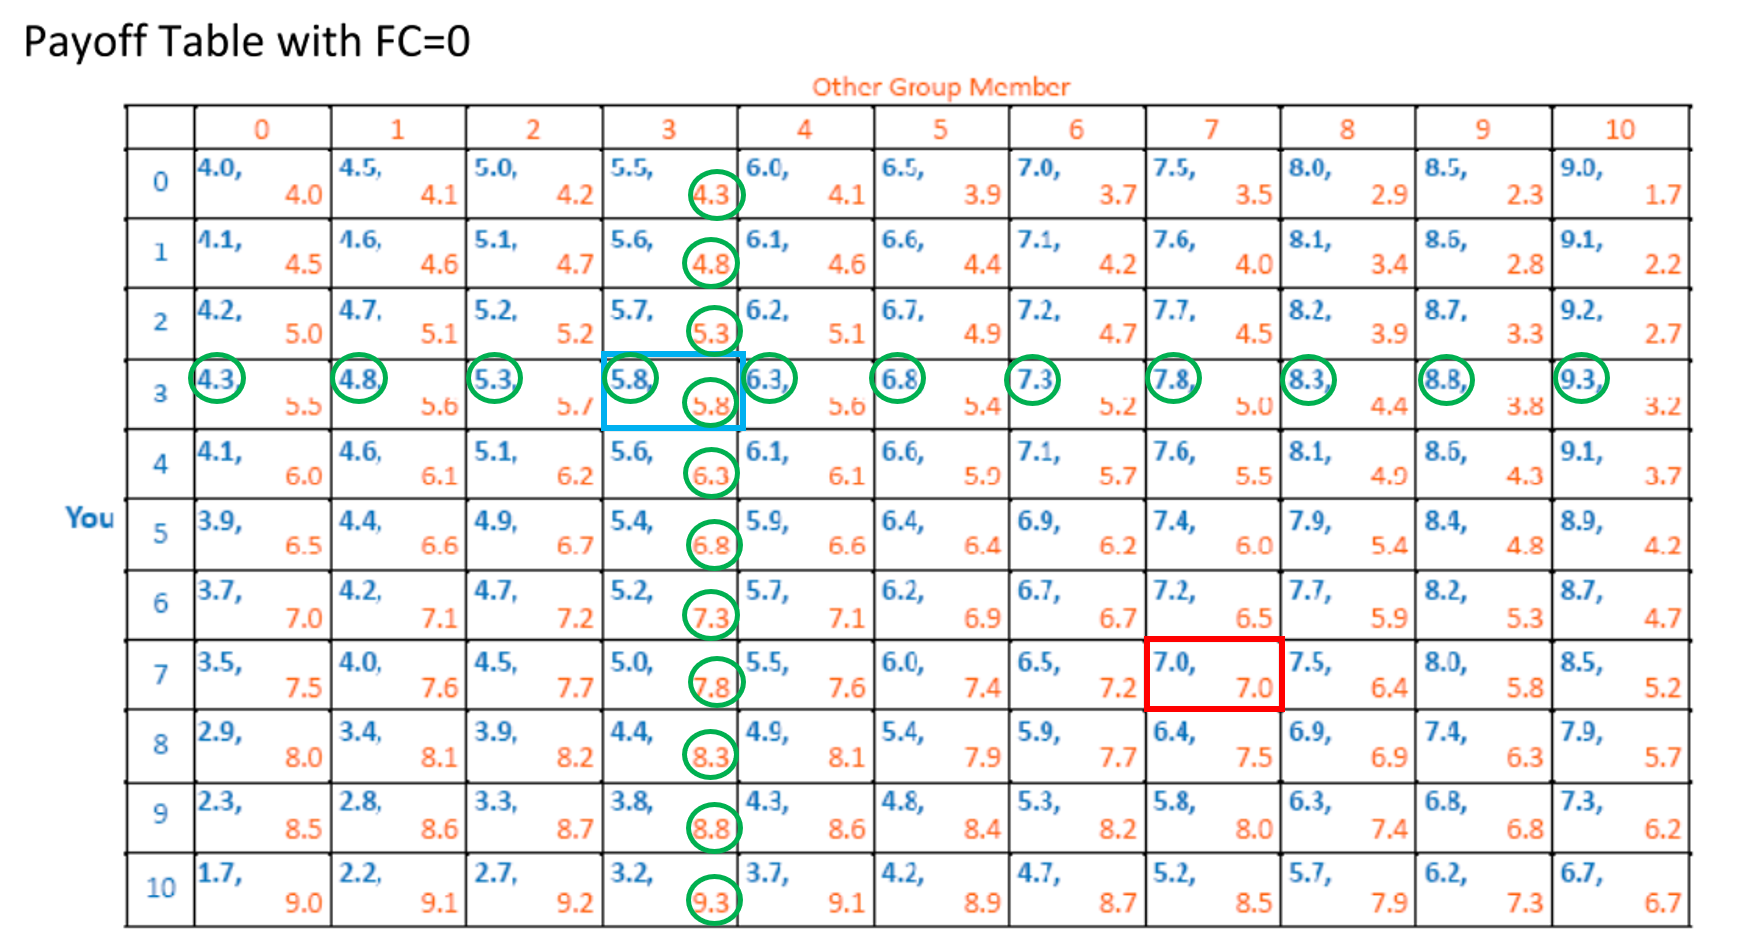
\includegraphics[width = 16cm]{0605kato/payoff_FC0.png}
        \caption{Payoff Table with $FC = 0$}
        \label{payoff FC0}
    \end{figure}

    \begin{figure}[H]
        \centering
        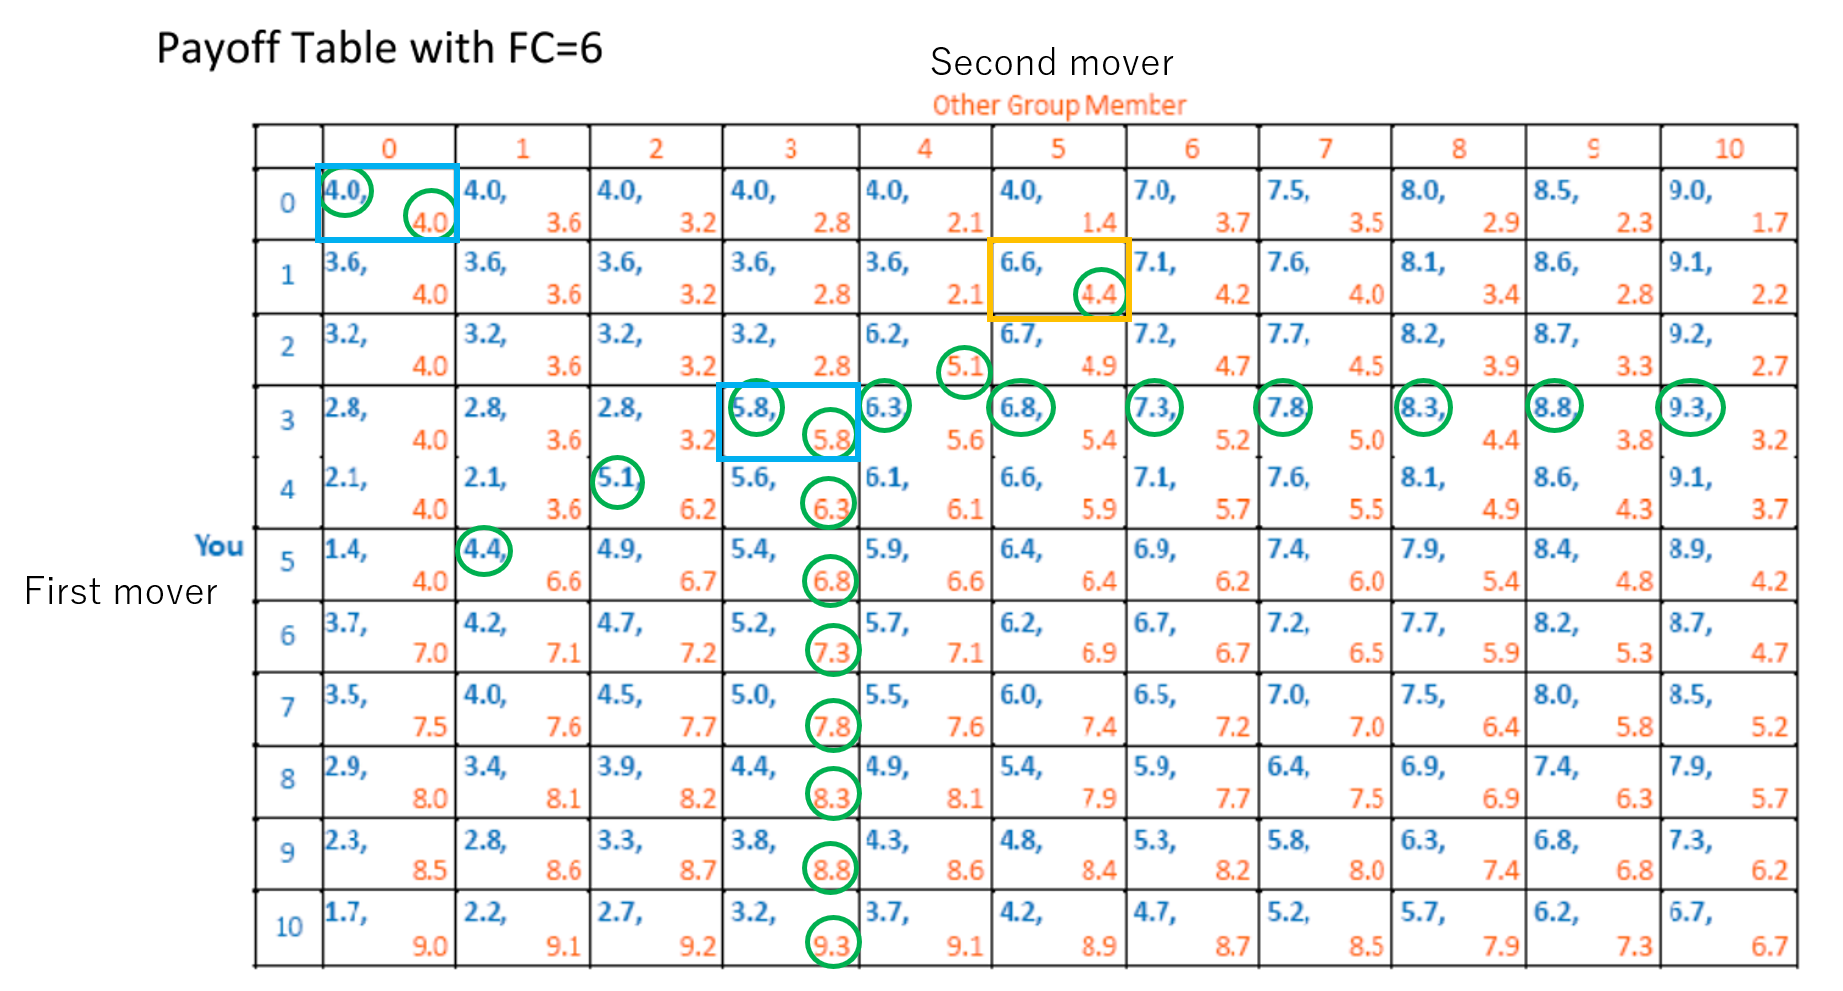
\includegraphics[width = 16cm]{0605kato/payoff_FC6.png}
        \caption{Payoff Table with $FC = 6$}
        \label{payoff FC6}
    \end{figure}

    \begin{figure}[H]
        \centering
        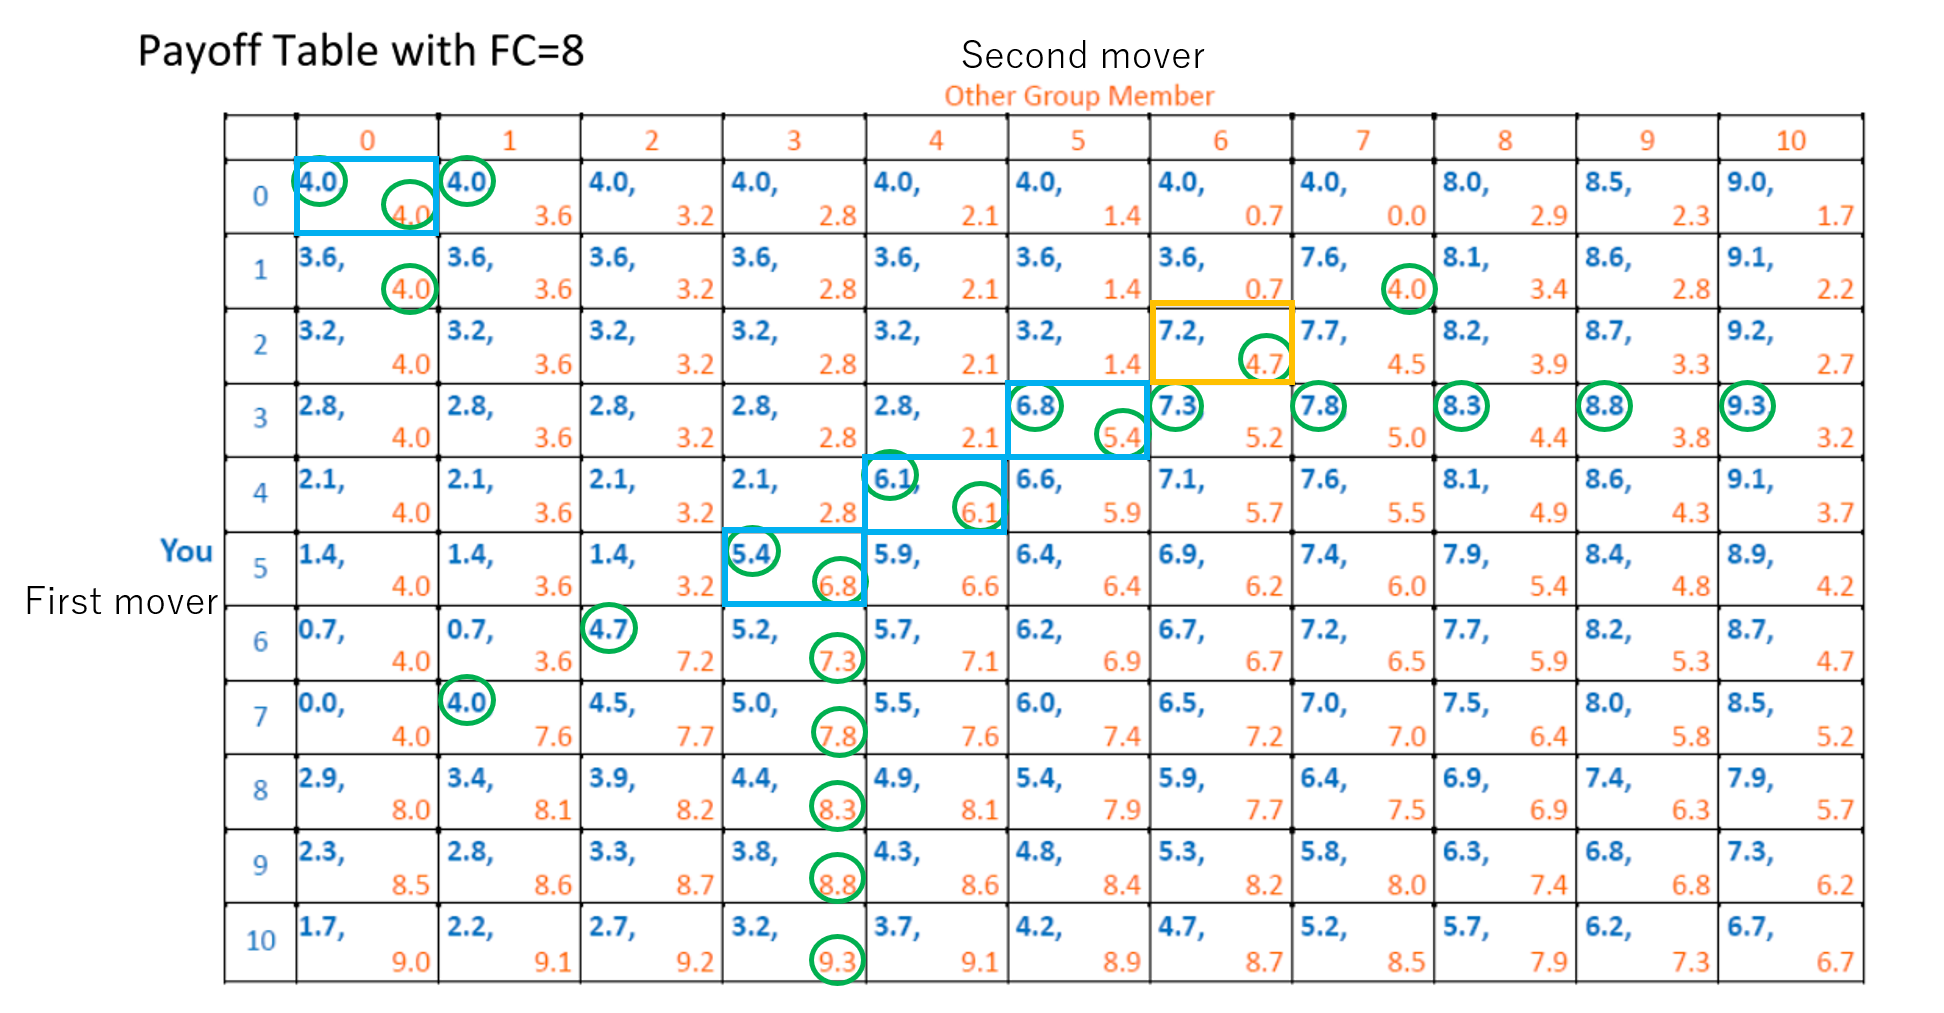
\includegraphics[width = 16cm]{0605kato/payoff_FC8.png}
        \caption{Payoff Table with $FC = 8$}
        \label{payoff FC8}
    \end{figure}

    \subsection{Procedure}

    \begin{itemize}
        \item Locate: the Pittsburgh Experimental Economics Laboratory at the University of Pittsburgh.
        \item With 14 participants per session a total of 224 undergraduate students participated in the study.
        \item Procedure:
        \begin{enumerate}
            \item Distributes instructions and payoff table
            \item The instructions were read out loud and a short quiz was given to gauge the participants' understanding.
            \item Distributes the solution key and an experimenter explains it.
            \item Play 14 rounds of the public goods game. In each round, each participant was randomly paired with another participant.
        \end{enumerate}
        \item Payoff = (Random selected 3 rounds) + (\$5 show-up fee)
    \end{itemize}

    
    \section{Results}

    \subsection{Hypothesis 1: Without fixed costs, No effect of the sequential play on contributions}  

    \begin{figure}[H]
        \centering
        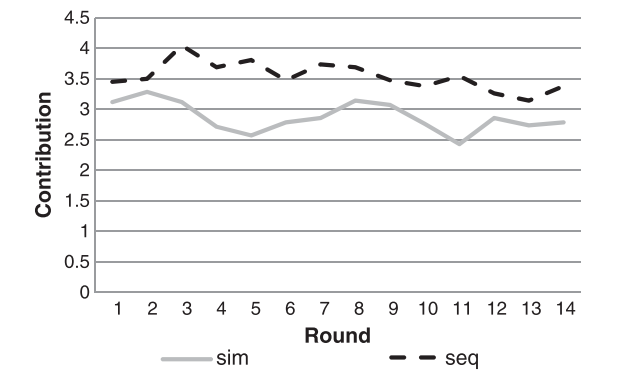
\includegraphics[width = 10cm]{0605kato/h1.png}
        \caption{Mean individual contributions without fixed costs}
        \label{hypo1}
    \end{figure}

    \begin{itemize}
        \item Reject hypothesis 1. When fixed costs are zero, sequential play increases contributions (figure \ref{hypo1}).
        \begin{itemize}
            \item A mean contribution of 2.87 units in the simultaneous game differs insignificantly from the prediction ($p = 0.382$).
            \item A mean contribution of 3.53 units in the sequential game differs significantly from the prediction ($p = 0.00$).
        \end{itemize}
        \item Possible explanation: Reciprocity
        \begin{itemize}
            \item When the first mover's contribution ranges between 0 and 3 units, the average second mover contribution is 2.99 units.
            \item When the first mover's contribution is more than 3 units, the average second mover contribution is 3.80 units.
        \end{itemize}
    \end{itemize}


    \subsection{Hypothesis 2: Mean contribution with 6 fixed costs are smaller than without fixed costs (simultaneous game)}

    \begin{itemize}
        \item By the introduction of fixed costs, an inefficient equilibrium with zero contribution emerges along with the previous one. If the inefficient equilibrium is played with some positive probability, average contributions are predicted to be lower with fixed costs of six.
    \end{itemize}

    \begin{figure}[H]
        \centering
        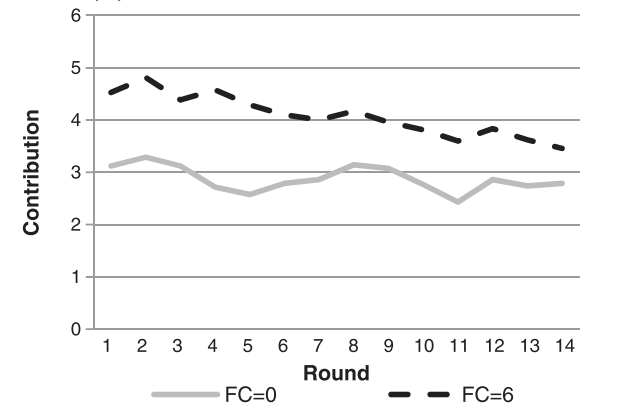
\includegraphics[width = 10cm]{0605kato/h2.png}
        \caption{Mean individual contributions with fixed costs of zero and six}
        \label{hypo2}
    \end{figure}

    \begin{figure}[H]
        \centering
        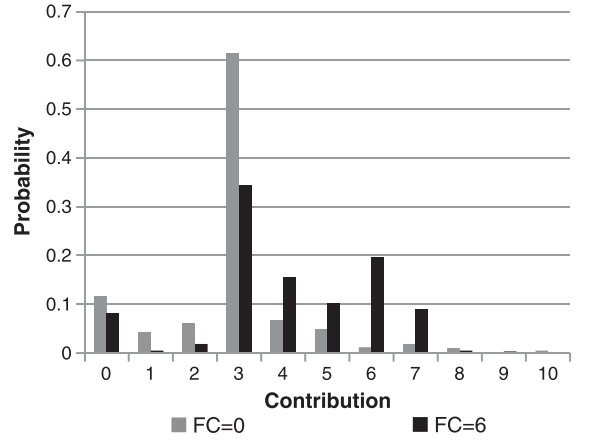
\includegraphics[width = 10cm]{0605kato/h2_add.png}
        \caption{Distributions of contributions with fixed costs of zero and six}
        \label{hypo2 add}
    \end{figure}

    \begin{itemize}
        \item Reject hypothesis 2. the introduction of low fixed costs is found to significantly increase contributions rather than decreasing contributions.
        \begin{itemize}
            \item Regression shows that introducing a fixed cost of six increases individual contributions by 1.20 units all else equal.
        \end{itemize}
        \item Possible explanation: Strategic uncertainty
        \begin{itemize}
            \item Consider beliefs that only place weight on the partner selecting an action associated with the two Nash equilibria: 0 or 3 units.
            \item If the likelihood of being matched with a zero contributor lies in the range of 40 to 80\%, the best response is to contribute 6 units.
            \item In fact, the second most common strategy is to contribute 6 units rather than 0 units (figure \ref{hypo2 add}).
            \item Observe learning effect. During the first seven rounds, 3 and 6 unit contributions each account for 25\% of all play. These numbers change for the latter half of the experiment, with 44\% of all contributions at three and only 14\% at six.
        \end{itemize}
    \end{itemize}

    \subsection{Hypothesis 3: Sequential play increases contributions with six fixed costs}

    \begin{figure}[H]
        \centering
        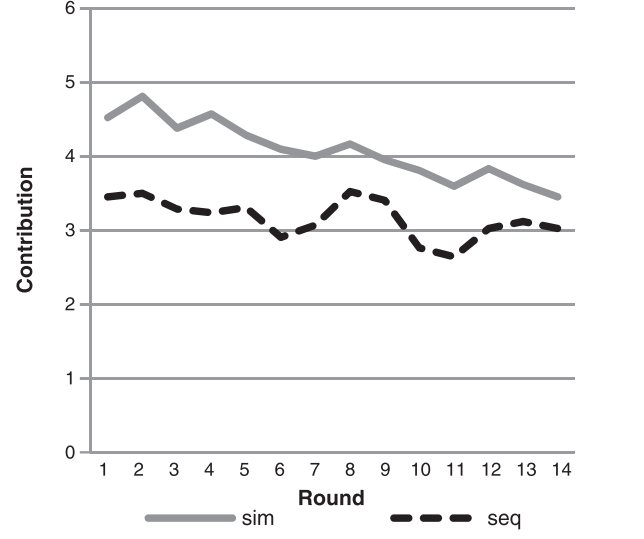
\includegraphics[width = 10cm]{0605kato/h3.png}
        \caption{Mean individual contributions with fixed costs six}
        \label{hypo3}
    \end{figure}

    \begin{itemize}
        \item Reject hypothesis 3. With fixed costs of six, sequential play decreases the mean contribution.
        \begin{itemize}
            \item Regression result shows that sequential play reduces individual contributions by almost 1 unit all else equal.
            \item We cannot reject that the average contribution of 3.16 in the sequential game equals the predicted mean contribution, that is, 3 units ($p = 0.380$).
        \end{itemize}
        \item Possible explanation: A reduce of strategic uncertainty
    \end{itemize}

    \begin{figure}[H]
        \centering
        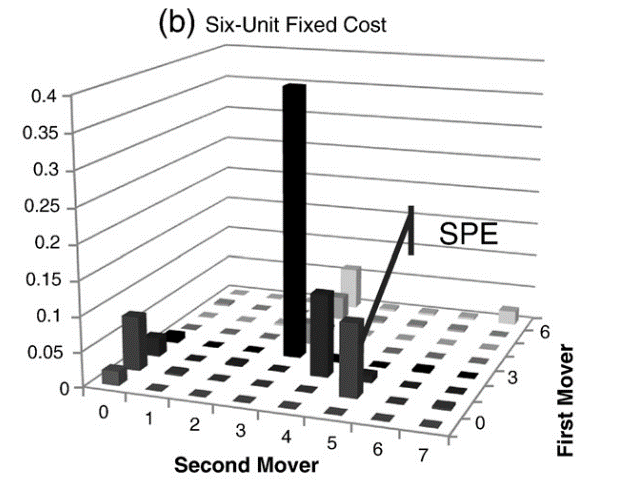
\includegraphics[width = 10cm]{0605kato/eqm_FC6.png}
        \caption{Equilibrium selection in the sequential game with fixed costs six}
        \label{eqm fc6}
    \end{figure}

    \begin{itemize}
        \item Although provision rates are 86\%, participants shy away from the highlighted subgame perfect equilibrium $(1,5)$. The most common equilibrium is $(3,3)$.
        \item Thus, first movers cannot take advantage. Indeed, first movers earn 7 cents less than second movers, however this difference is not significant $(p = 0.60)$.
        \item Second movers may view contribution of one out of six as more unfair.
    \end{itemize}

    \subsection{Hypothesis 4: With an eight-unit fixed cost, sequential play increases contributions}

    \begin{figure}[H]
        \centering
        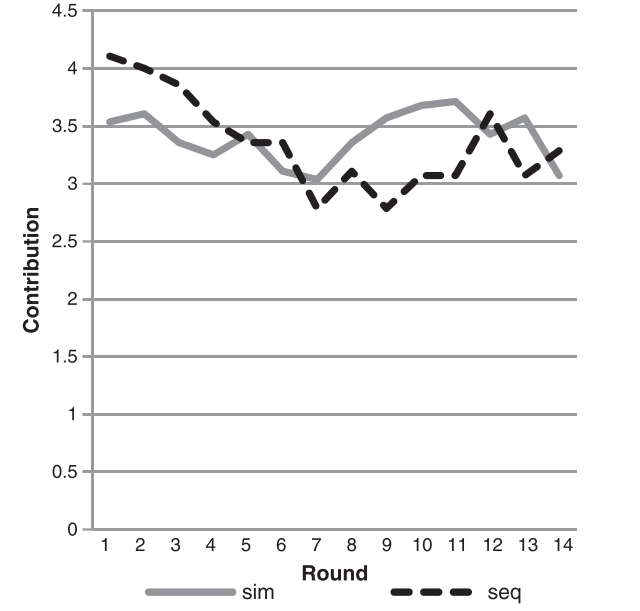
\includegraphics[width = 8cm]{0605kato/h4.png}
        \caption{Mean individual contributions with fixed costs eight}
        \label{hypo4}
    \end{figure}

    \begin{figure}[H]
        \centering
        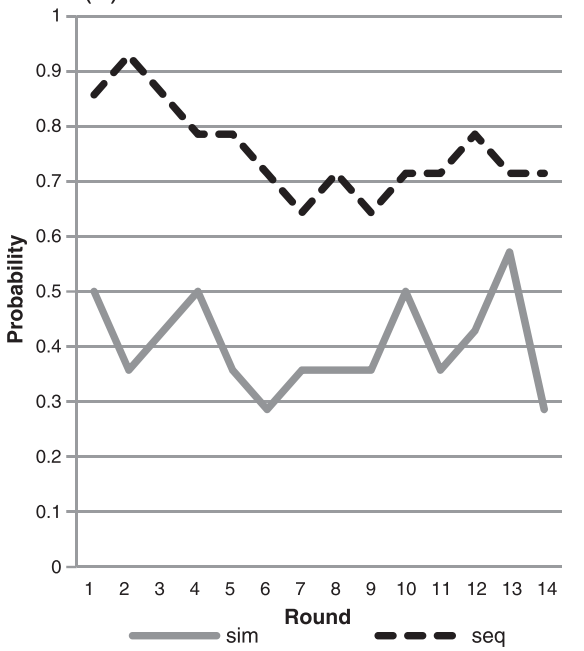
\includegraphics[width = 8cm]{0605kato/h4_add.png}
        \caption{Probability of provision with fixed costs eight}
        \label{hypo4 add}
    \end{figure}

    \begin{itemize}
        \item Reject hypothesis 4. Sequential play does not significantly increase individual contributions.
        \item However, \textit{sequential play increases round earnings by approximately \$1.20, a 27\% increase}.
        \begin{itemize}
            \item In the simultaneous game, a third of all contributions are at zero units.
            \item This result implies that the likelihood of providing the public good does increase substantially (see figure \ref{hypo4 add}).
        \end{itemize}
    \end{itemize}

    \begin{figure}[H]
        \centering
        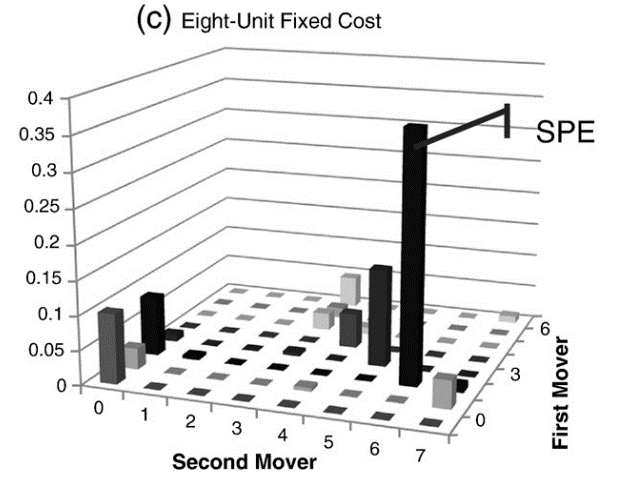
\includegraphics[width = 10cm]{0605kato/eqm_FC8.png}
        \caption{Equilibrium selection in the sequential game with fixed costs eight}
        \label{eqm fc8}
    \end{figure}

    \begin{itemize}
        \item Contrary to six units fixed costs, the most common equilibrium is the highlighted subgame perfect equilibrium of $(2,6)$.
        \item This leads to a significant and substantial first mover advantage. The earnings of first movers on average exceed those of the second movers by 87 cents. 
    \end{itemize}


    \section{Concluding Remarks}

    About the results, authors summarize as follows:

    \begin{quote}
        To summarize in the no and high fixed cost treatments behavior in both the sequential and simultaneous games is broadly consistent with the equilibrium predictions, however in the low-cost treatments we see substantial deviations in both the sequential and simultaneous games. On one hand strategic uncertainty appears to cause greater than predicted simultaneous giving when the fixed costs is low; on the other hand the tension associated with the substantial first mover advantage appears to move behavior away from the asymmetric subgame perfect equilibrium. (\citealp[p.425]{Bracha2011})
    \end{quote}

    They state implications from this experiment as follows:
    
    \begin{quote}
        ..., the introduction of fixed costs increases the first mover advantage inherent in the public good game, and a potential risk of sequential play is that provision may fail unless the fundraiser is successful in convincing initial contributors to donate a fair share (\citealp[p.426]{Bracha2011}).
    \end{quote}



    \biblio

\end{document}